
\documentclass[12pt]{exam}
\usepackage{amsthm}
\usepackage{libertine}
%\usepackage[utf8]{inputenc}
\usepackage[margin=1in]{geometry}
\usepackage{amsmath,amssymb}
\usepackage{multicol}
\usepackage[shortlabels]{enumitem}
\usepackage{siunitx}
\usepackage{cancel}
\usepackage{graphicx}
\graphicspath{{./}}
\usepackage{pgfplots}
\usepackage{hyperref}
\usepackage{listings}
\usepackage{tikz}
\usepackage{minted}
\def\code#1{\texttt{#1}}
\usepackage{amssymb}
\usepackage{xcolor}
% for plotting
\usepackage{pgfplots}
\pgfplotsset{compat=1.16}
\usepackage{tikz}
\usetikzlibrary{arrows.meta}


\newcommand{\quotebox}[1]
{
  \begin{center}
    \fcolorbox{white}{blue!15!gray!15}{
      \begin{minipage}{0.7\linewidth}\vspace{10pt}
        \center
        \begin{minipage}{0.8\linewidth}{\space\Huge``}{\setlength{\parindent}{1.5em}#1}{\hspace{1.5em}\break\null\Huge\hfill''}
        \end{minipage}
        \smallbreak
      \end{minipage}
    }
\end{center}
}

%\DeclareUnicodeCharacter{2212}{-}


\let\oldemptyset\emptyset
\let\emptyset\varnothing

\hypersetup{
    colorlinks=true,
    linkcolor=blue,
    filecolor=magenta,      
    urlcolor=cyan,
    pdftitle={Overleaf Example},
    pdfpagemode=FullScreen,
    }
    
\urlstyle{same}

\pgfplotsset{width=10cm,compat=1.9}
\usepgfplotslibrary{external}
\tikzexternalize

\newcommand{\class}{Math 415} % This is the name of the course 
\newcommand{\examnum}{Homework-10} % This is the name of the assignment
\newcommand{\examdate}{Nov 27} % This is the due date
\newcommand{\timelimit}{}

\newcommand{\BO}{\mathcal{O}}




\begin{document}
\pagestyle{plain}
\thispagestyle{empty}

\noindent
\begin{tabular*}{\textwidth}{l @{\extracolsep{\fill}} r @{\extracolsep{6pt}} l}
\textbf{\class} & \textbf{Name:} & \textit{Zhenzhao Tu}\\ %Your name here instead, obviously 
\textbf{\examnum} &&\\
\textbf{\examdate} &&\\
\end{tabular*}\\
\rule[2ex]{\textwidth}{2pt}
% --

\section*{Problem 1}

Consider the van der Pol oscillator $\ddot{x} + \mu(x^2 − 1)\dot{x} + x = a$ for real parameters $\mu$ and $a$. Find the curves in the $(\mu,a)$-space at which a Hopf bifurcation occurs, for what $(x,\dot{x})$ does it occur at?

\subsection*{Solution:}
Let $y = \dot{x}$, then we have the system
\[ \begin{cases}
\dot{x} = y \\
\dot{y} = a - x - \mu(x^2 - 1)y
\end{cases} \]

When $\dot{x} = \dot{y} = 0$, we can find nullclines $y = a-x/\mu(x^2 - 1)$ and $y = 0$. The intersection of these two nullclines is $(x,y) = (a, 0)$ which is the only fixed point of the system. The Jacobian matrix of the system is
\[ J(x,y) = \begin{bmatrix}
0 & 1 \\
-1 - 2\mu xy & -\mu(x^2 - 1)
\end{bmatrix}_{(a,0)} = \begin{bmatrix}
0 & 1 \\
-1 & -\mu(a^2 - 1)
\end{bmatrix} \]

The $\tau = \text{tr}(J) = -\mu(a^2 - 1)$ and $\Delta = \text{det}(J) = 2a\mu y+1$. The Hopf bifurcation occurs when $\tau = 0$ and $\Delta > 0$. Thus, the Hopf bifurcation occurs at $a = \pm 1$. Thus the Hopf bifurcation occurs at $(x,y) = (\pm 1, 0)$.


\section*{Problem 2}
Consider the system
\[ \begin{cases}
	\dot{x} = x[x(1-x) - y] \\
	\dot{y} = y(x - a)
\end{cases} \]
where $x \geq 0$ is the dimensionless population of the prey, $y \geq 0$ is the dimensionless population of the predator, and $a \geq 0$ is a control parameter.

\begin{enumerate}[(a)]
	\item Sketch the nullclines in the first quadrant $(x, y \geq 0)$. \\
	Here is the nullclines in the first quadrant.
	\begin{figure}[ht]
		\centering
		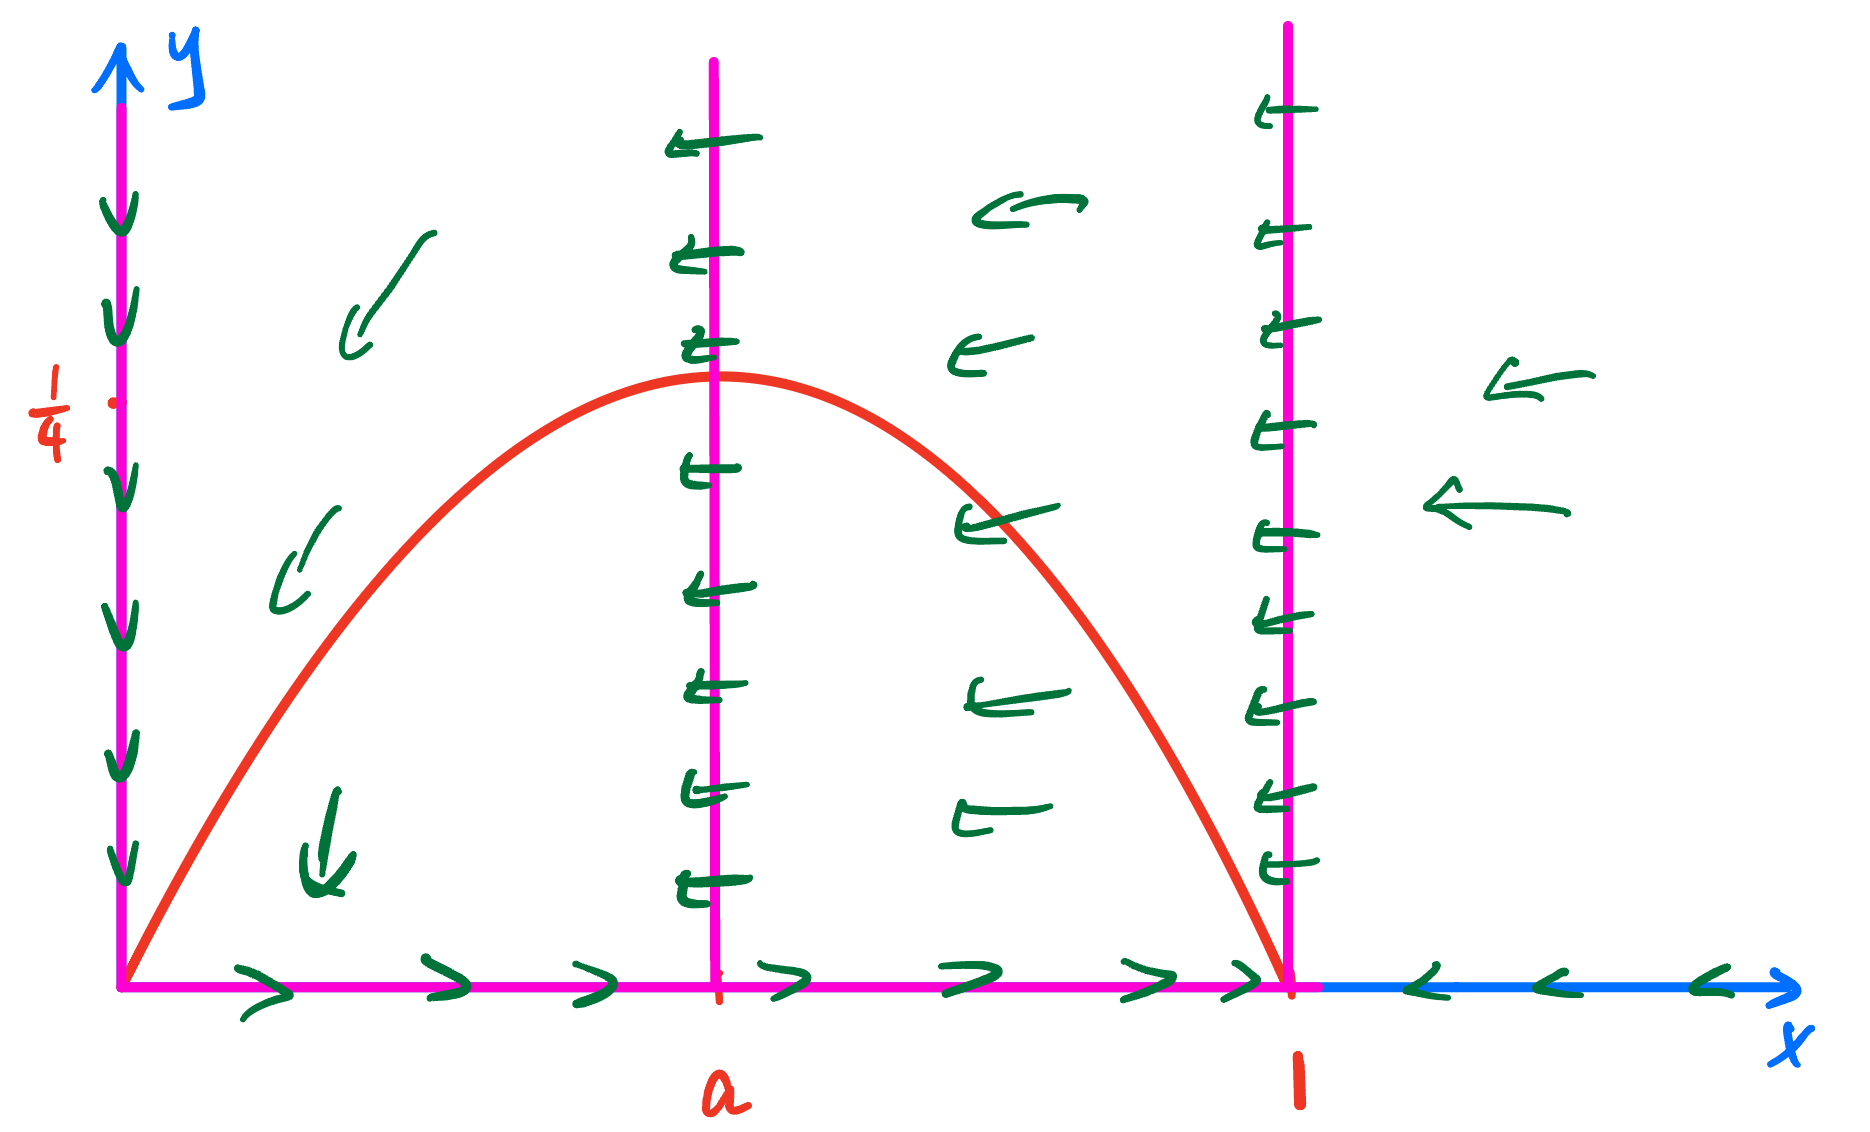
\includegraphics[width=0.7\linewidth]{2a.jpeg}
		\caption{Nullclines in the first quadrant}
		\label{fig:2a}
	\end{figure}

	When $\dot{x} = \dot{y} = 0$, we have nullclines $x = 0$, $y = 0$, $x = 1$, and $x=a$. Thus we have three fixed points $(x,y) = (0,0)$, $(1,0)$, and $(a,a-a^2)$. The Jacobian matrix of the system is
	\[ J(x,y) = \begin{bmatrix}
		2x(1-x) - y & -x \\
		y & x-a
	\end{bmatrix} \]

	\item Show that the fixed points and classify them.
	From the Jacobian matrix, we have
	\[ J(0,0) = \begin{bmatrix}
		0 & 0 \\
		0 & -a
	\end{bmatrix}, \quad J(1,0) = \begin{bmatrix}
		-1 & -1 \\
		0 & 1-a
	\end{bmatrix}, \quad J(a,a-a^2) = \begin{bmatrix}
		a-2a^2 & -a \\
		a-a^2 & 0
	\end{bmatrix} \]
	\begin{enumerate}[(i)]
		\item $(0,0)$: $\tau = -a$, $\Delta = 0$, thus the fixed point is line of stable nodes.
		\item $(1,0)$: $\tau = -a$, $\Delta = a-1$. When $a < 1$, the fixed point is a saddle point. When $a = 1$, the fixed point is a line of stable nodes. When $a > 1$, the fixed point is a stable node.
		\item $(a,a-a^2)$: $\tau = a-2a^2$, $\Delta = a^2 - 2a^3$. When $a=0$, the fixed point is uniform motion. When $0 < a < 1/2$, the fixed point is an unstable spiral. When $a = 1/2$, the fixed point is also uniform motion. When $a > 1/2$, the fixed point is a saddle point.	
	\end{enumerate}

	\item Sketch the phase portrait for $a >1$. What happens to the predators as $t \to \infty$? \\
		Here is the phase portrait for $a > 1$ when $a = 2$.
		\begin{figure}[H]
			\centering
			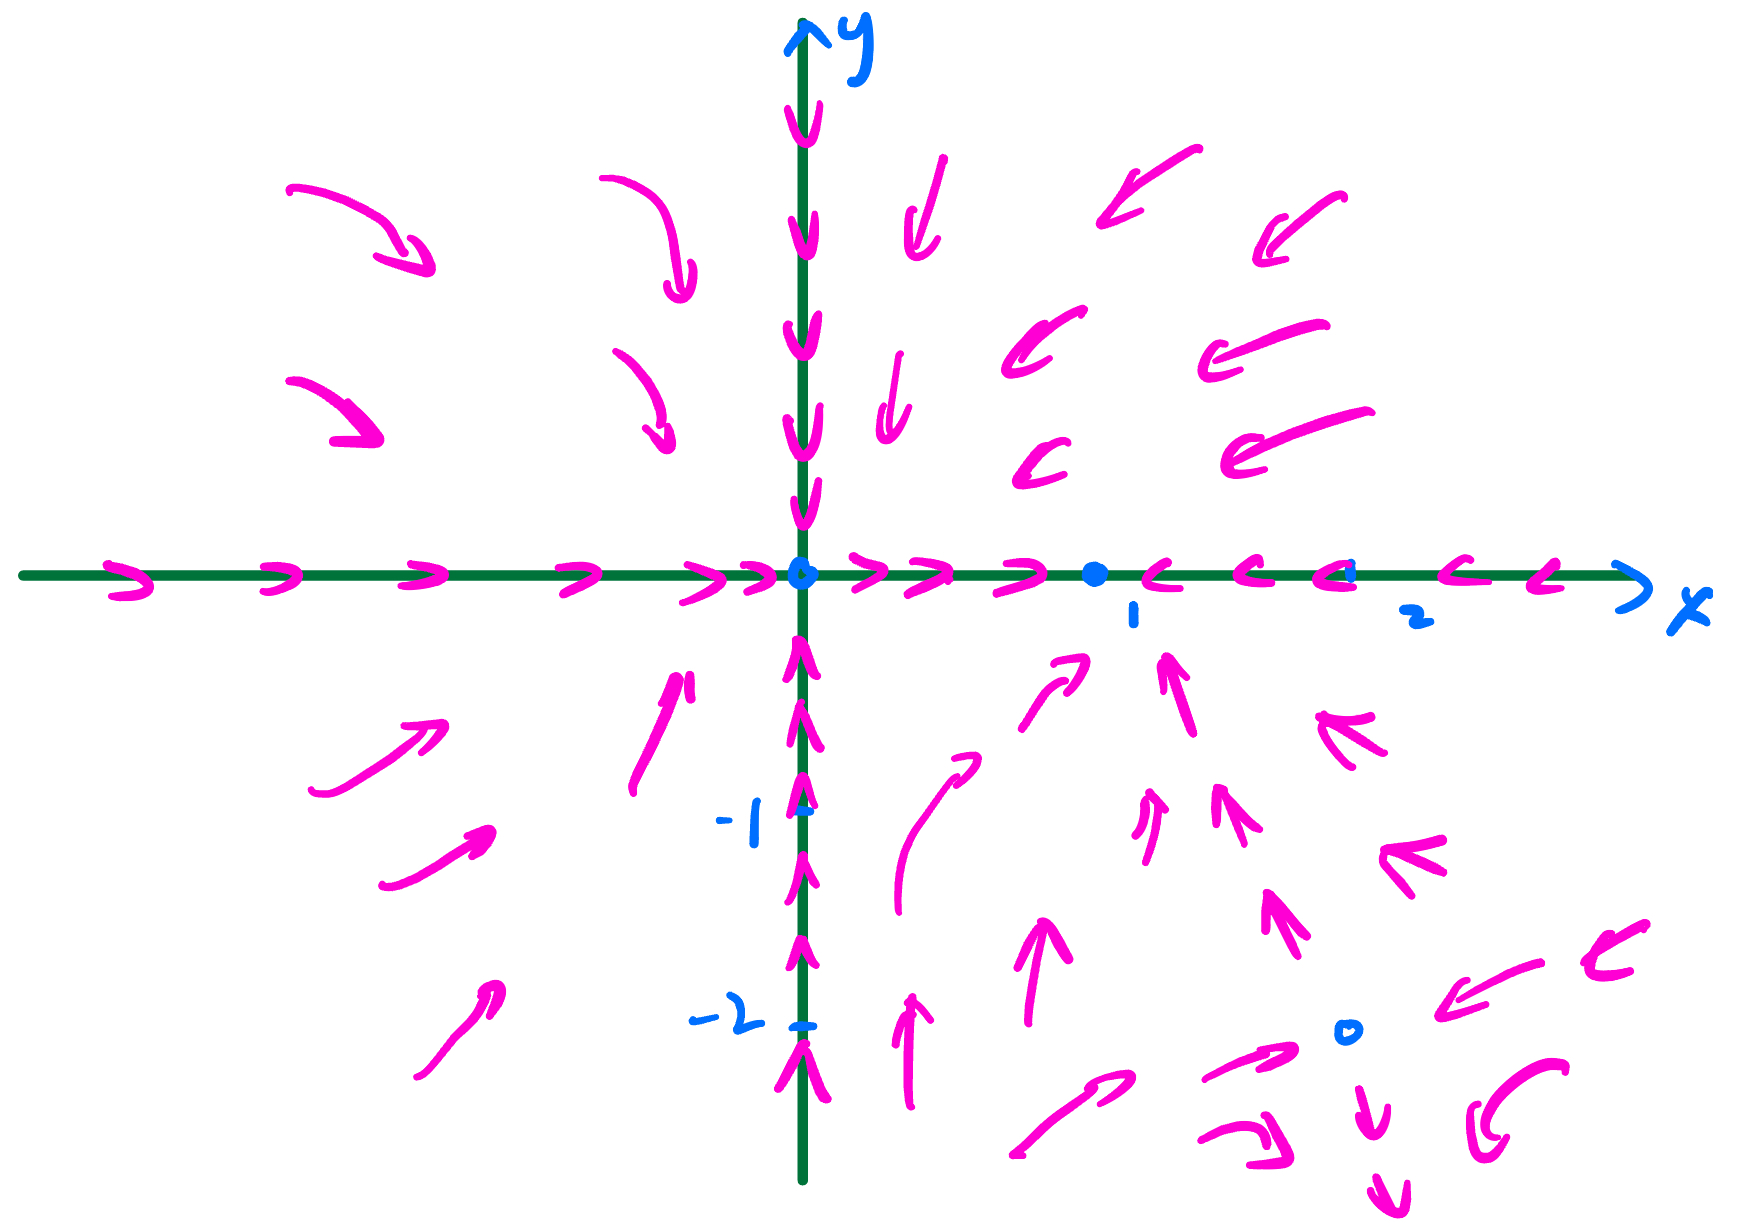
\includegraphics[width=0.8\linewidth]{2c.jpeg}
			\caption{Phase portrait for $a = 2$}
			\label{fig:2c}
		\end{figure}

		As $t \to \infty$, the predators will go to extinction and the prey will go to $1$.
	
	\item What type of bifurcation occurs at $a = 1$? \\
	At $a = 1$, the fixed point $(1,0)$ changes from a saddle point to a stable node. Thus, the bifurcation is a saddle-node bifurcation.

	\item At what value of $a$ does the Hopf bifurcation occur? 
	\[ \tau = a-2a^2 = 0 \implies a = 0, \frac{1}{2} \]


\end{enumerate}


\section*{Problem 3}
Consider the Lorenz system
\[ \begin{cases}
	\dot{x} = \sigma(y-x) \\
	\dot{y} = x(r - z) - y \\
	\dot{z} = xy - bz
\end{cases} \]

\begin{enumerate}
	\item First find the Jacobian matrix $J(x,y,z)$ of the system at fixed point.

	\[ J(x,y,z) = \begin{bmatrix}
		-\sigma & \sigma & 0 \\
		r-z & -1 & -x \\
		y & x & -b
	\end{bmatrix}_{(\pm \sqrt{b(r-1)}, \pm \sqrt{b(r-1)}, r-1)} \]
	Then
	\[ \begin{bmatrix}
		-\sigma & \sigma & 0 \\
		0 & -1 & \pm \sqrt{b(r-1)} \\
		\pm \sqrt{b(r-1)} & \pm \sqrt{b(r-1)} & -b
	\end{bmatrix} \]
	Thus, the $\det(J - \lambda I) = 0$ is	
	\[ \begin{vmatrix}
		-\sigma - \lambda & \sigma & 0 \\
		0 & -1 - \lambda & \pm \sqrt{b(r-1)} \\
		\pm \sqrt{b(r-1)} & \pm \sqrt{b(r-1)} & -b - \lambda
	\end{vmatrix} = 0 \]
	By the general formula of characteristic polynomial
	\[ \lambda^3 - Tr(J)\lambda^2 + (J_{11}J_{22} + J_{11}J_{33} + J_{22}J_{33} - J_{12}J_{21} - J_{13}J_{31} - J_{23}J_{32})\lambda - \det(J) = 0 \]
	we have
	\[ \lambda^3 + (\sigma + 1 + b)\lambda^2 + (r+\sigma)b\lambda + 2b\sigma (r-1) = 0 \]

	\item For eigenvalue $\lambda = i \omega$, we can plug into the characteristic polynomial and get
	\[ (i\omega)^3 + (\sigma + 1 + b)(i\omega)^2 + (r+\sigma)b(i\omega) + 2b\sigma (r-1) = 0 \]
	That gives us in imaginary part and real part equal to zero
	\[ [2b\sigma (r-1) - (\sigma + 1 + b)\omega^2] + [b(r+\sigma)\omega - i \omega^3] = 0 \]
	Since imaginary part and real part are equal to zero, we have
	\[ 2b\sigma (r-1) = (\sigma + 1 + b)\omega^2, \quad b(r+\sigma)\omega = \omega^3  \]
	Thus, we have
	\[ \frac{2b\sigma (r-1)}{1+\sigma+b} = \omega^2, \quad b(r+\sigma) = \omega^2 \]
	Then we can solve for $r$,
	\[ r = \frac{\sigma (\sigma + b + 3)}{\sigma - b - 1} \]
	when $\sigma > b + 1$. Since this pair of eigenvalues are zero, Hopf bifurcation occurs at $r_H = \sigma (\sigma + b + 3)/(\sigma - b - 1)$.

	\item Since the $\tau$ of the system is $-\sigma - 1 - b$ and the sum of two pairs of eigenvalues is zero, thus the third eigenvalue is $\lambda_3 = -(\sigma + 1 + b)$. 




\end{enumerate}












\end{document}

